\documentclass[tikz,border=2pt]{standalone}
\usepackage{amsmath,amssymb}
\usepackage{tikz}
\usetikzlibrary{arrows.meta}

\begin{document}
% For a C^3 function the eight third-order partials of f(x,y) collapse to four: only how
% many times each variable is used matters, not the order.
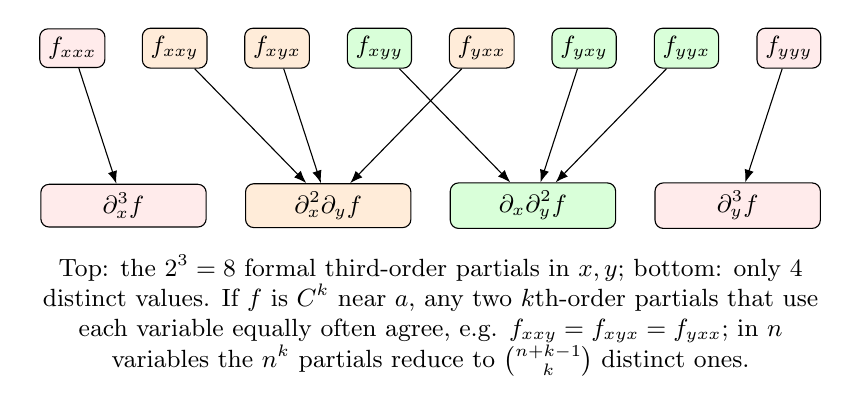
\begin{tikzpicture}[every node/.style={font=\small}, >={Latex[length=1.6mm]}, lvl/.style={draw, rounded corners=3pt, fill=blue!8, inner sep=3pt}]
	\node[lvl, fill=red!8] (a1) at (-4.55,0) {$f_{xxx}$};
	\node[lvl, fill=orange!15] (a2) at (-3.25,0) {$f_{xxy}$};
	\node[lvl, fill=orange!15] (a3) at (-1.95,0) {$f_{xyx}$};
	\node[lvl, fill=green!15] (a4) at (-0.65,0) {$f_{xyy}$};
	\node[lvl, fill=orange!15] (a5) at (0.65,0) {$f_{yxx}$};
	\node[lvl, fill=green!15] (a6) at (1.95,0) {$f_{yxy}$};
	\node[lvl, fill=green!15] (a7) at (3.25,0) {$f_{yyx}$};
	\node[lvl, fill=red!8] (a8) at (4.55,0) {$f_{yyy}$};
	\node[lvl, fill=red!8, minimum width=2.1cm] (b1) at (-3.9,-2.0) {$\partial_x^3f$};
	\node[lvl, fill=orange!15, minimum width=2.1cm] (b2) at (-1.3,-2.0) {$\partial_x^2\partial_yf$};
	\node[lvl, fill=green!15, minimum width=2.1cm] (b3) at (1.3,-2.0) {$\partial_x\partial_y^2f$};
	\node[lvl, fill=red!8, minimum width=2.1cm] (b4) at (3.9,-2.0) {$\partial_y^3f$};
	\draw[->] (a1) -- (b1);
	\draw[->] (a2) -- (b2); \draw[->] (a3) -- (b2); \draw[->] (a5) -- (b2);
	\draw[->] (a4) -- (b3); \draw[->] (a6) -- (b3); \draw[->] (a7) -- (b3);
	\draw[->] (a8) -- (b4);
	\node[anchor=north, align=flush center, text width=10cm] at (0,-2.5) {Top: the $2^3=8$ formal third-order partials in $x,y$; bottom: only $4$ distinct values. If $f$ is $C^k$ near $a$, any two $k$th-order partials that use each variable equally often agree, e.g. $f_{xxy}=f_{xyx}=f_{yxx}$; in $n$ variables the $n^k$ partials reduce to $\binom{n+k-1}{k}$ distinct ones.};
\end{tikzpicture}
\end{document}
